\documentclass{article}

\usepackage[a4paper, total={7.3in, 10.3in}]{geometry}
\usepackage{amsmath}
\usepackage{amsfonts}
\usepackage{amssymb}
\usepackage{tikz}
\usetikzlibrary{arrows.meta, positioning}
\usepackage{graphicx}
\graphicspath{{screenshots/}}


\title{TinyML and Efficient AI Computing MIT Course}
\author{\textbf{Hariprashad Ravikumar}} 
\date{}

\begin{document}
\maketitle

This document contains the lecture notes for the TinyML and Efficient AI Computing MIT course, alongside older personal machine learning notes and mathematical derivations.

\tableofcontents
\pagebreak


\section{TinyML and Efficient AI Computing}

\subsection{Lecture 2 - Basics of Neural Networks}

\begin{center}
    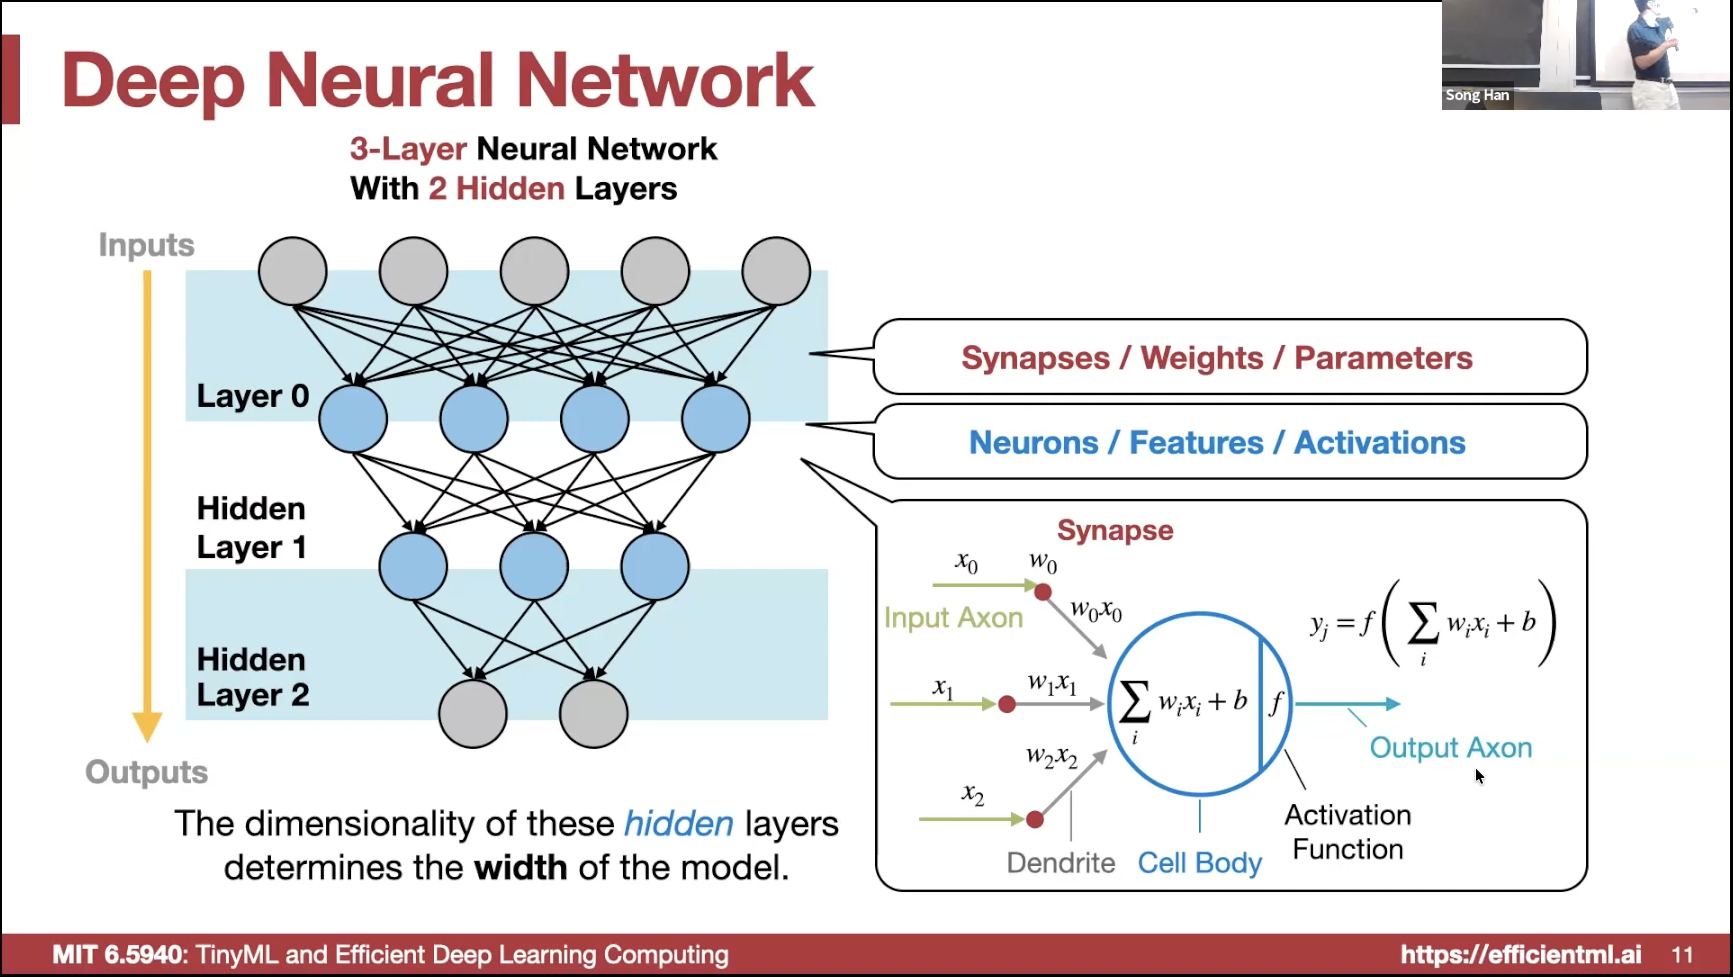
\includegraphics[width=\textwidth,height=0.3\textheight,keepaspectratio]{screenshot_1.png}
    
    \vspace{0.5cm}
    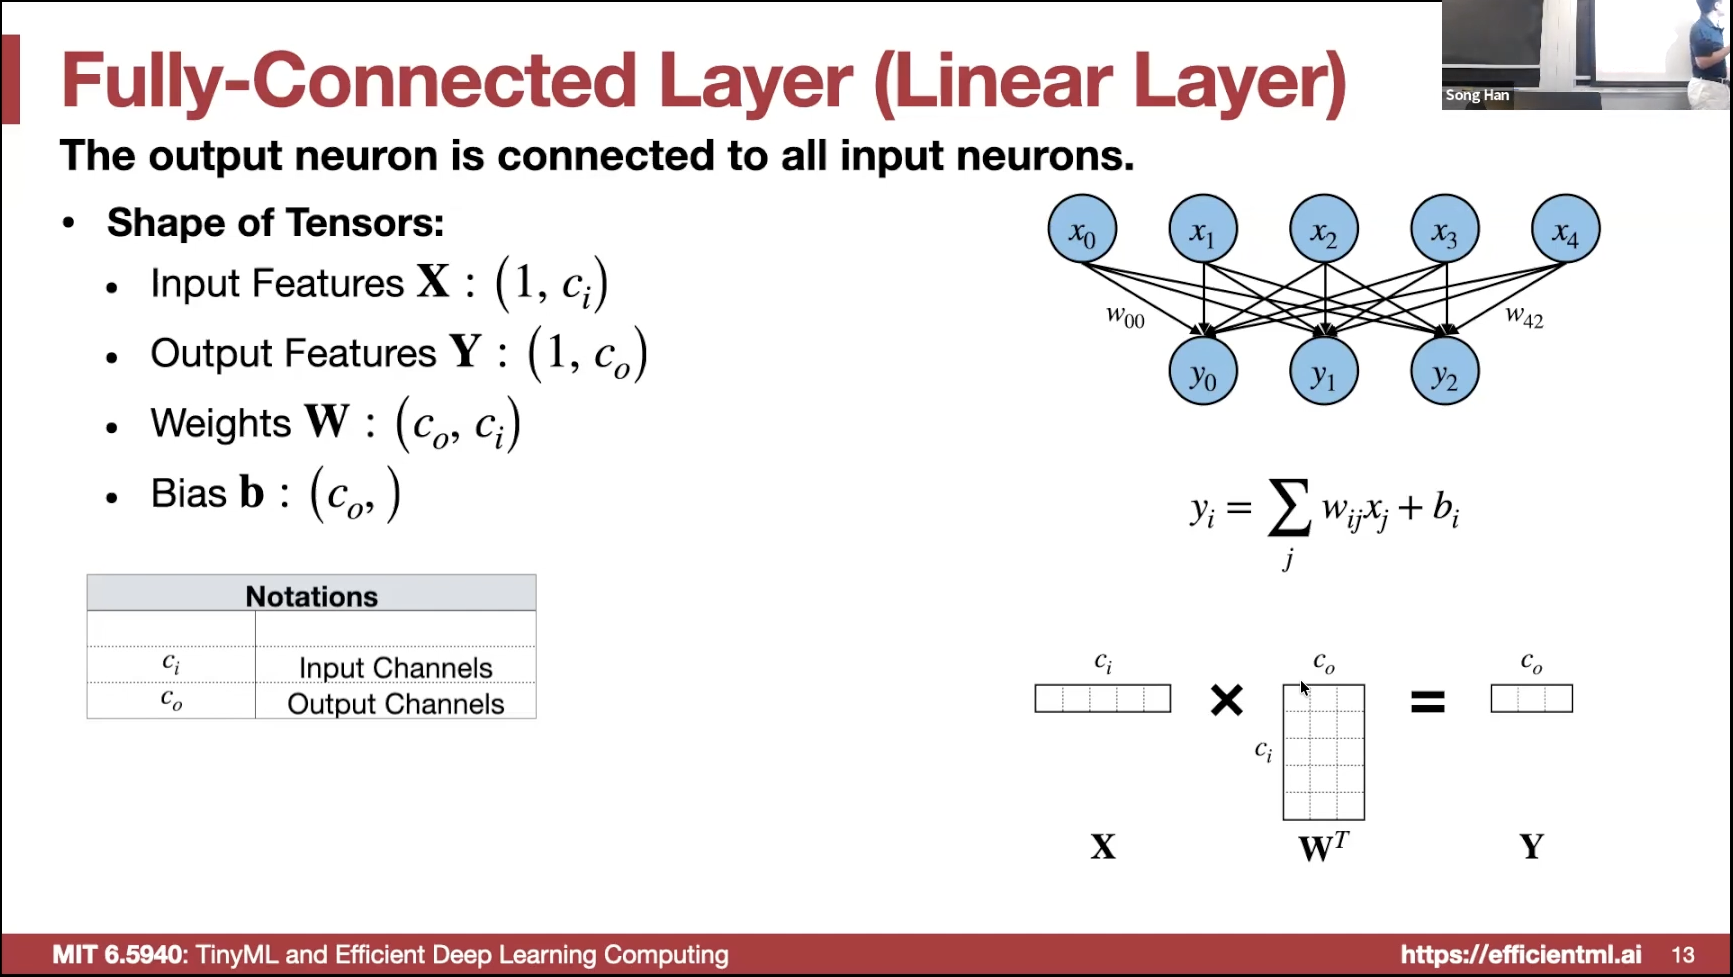
\includegraphics[width=\textwidth,height=0.3\textheight,keepaspectratio]{screenshot_2.png}
\end{center}

\pagebreak

\section{Hari's personal note on Neural Networks}

\section*{A Simple Neural Network}

\begin{figure}[htbp]
  \centering
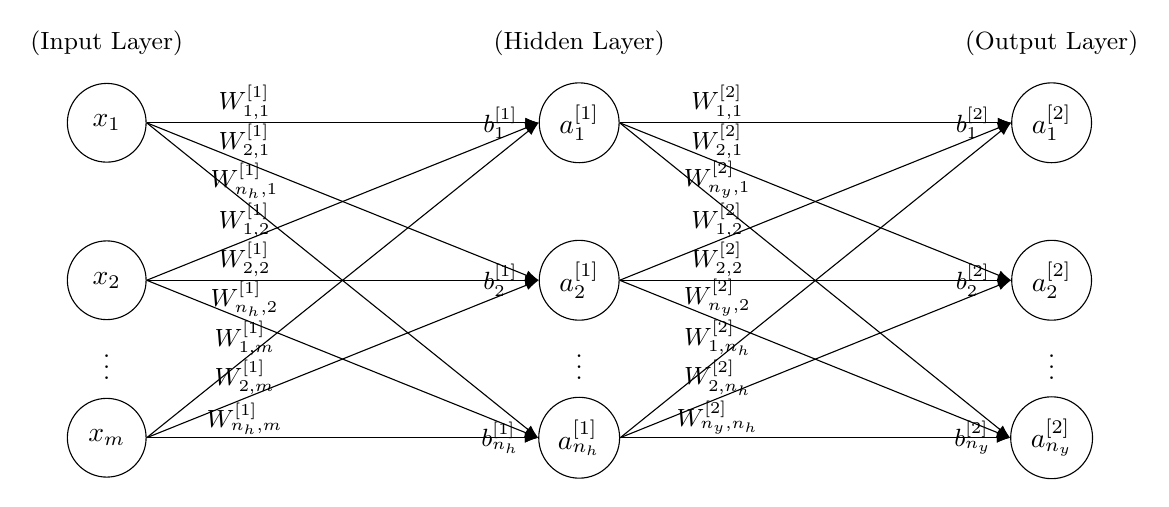
\begin{tikzpicture}[
  neuron/.style={circle, draw, minimum size=1cm},
  labelnode/.style={font=\small, inner sep=1pt},
  >=Latex
]
  %------------------------------------------------------------
  %  PARAMETERS
  %------------------------------------------------------------
  \def\xsep{6cm}    % horizontal separation between layers
  \def\yA{2cm}      % gap between Row 1 and Row 2
  \def\yB{1cm}      % gap between Row 2→Row 3 and Row 3→Row 4

  %------------------------------------------------------------
  %  ROW 1 (y=0):  x_1,  a^{[1]}_1,  a^{[2]}_1
  %------------------------------------------------------------
  \node[neuron] (X1)  at (0,0)              {$x_{1}$};
  \node[neuron] (A11) at (\xsep,0)          {$a^{[1]}_{1}$};
  \node[neuron] (A21) at (2*\xsep,0)        {$a^{[2]}_{1}$};

  %------------------------------------------------------------
  %  ROW 2 (y=-\yA):  x_2,  a^{[1]}_2,  a^{[2]}_2
  %------------------------------------------------------------
  \node[neuron] (X2)  at (0,-\yA)           {$x_{2}$};
  \node[neuron] (A12) at (\xsep,-\yA)       {$a^{[1]}_{2}$};
  \node[neuron] (A22) at (2*\xsep,-\yA)     {$a^{[2]}_{2}$};

  %------------------------------------------------------------
  %  ROW 3 (y=-(\yA+\yB)):  vertical dots “\vdots”
  %------------------------------------------------------------
  \node[labelnode] (Xdots) at (0,-\yA-\yB)       {$\vdots$};
  \node[labelnode] (Hdots) at (\xsep,-\yA-\yB)   {$\vdots$};
  \node[labelnode] (Odots) at (2*\xsep,-\yA-\yB){$\vdots$};

  %------------------------------------------------------------
  %  ROW 4 (y=-(\yA+2*\yB)):  x_m,  a^{[1]}_{n_h},  a^{[2]}_{n_y}
  %------------------------------------------------------------
  \node[neuron] (Xm)  at (0,-\yA-2*\yB)        {$x_{m}$};
  \node[neuron] (A1n) at (\xsep,-\yA-2*\yB)     {$a^{[1]}_{n_{h}}$};
  \node[neuron] (A2n) at (2*\xsep,-\yA-2*\yB)   {$a^{[2]}_{n_{y}}$};

  %------------------------------------------------------------
  %  LAYER TITLES
  %------------------------------------------------------------
  \node[labelnode, above=0.3cm of X1 ]  {(Input Layer)};
  \node[labelnode, above=0.3cm of A11]  {(Hidden Layer)};
  \node[labelnode, above=0.3cm of A21]  {(Output Layer)};

  %------------------------------------------------------------
  %  WEIGHTS:  Input → Hidden  (W^{[1]}_{j,i})
  %------------------------------------------------------------
  \foreach \i/\Xin in {1/X1, 2/X2, m/Xm} {
    \foreach \j/\Hin in {1/A11, 2/A12, n_h/A1n} {
      \draw[->]
        (\Xin.east)
        -- node[labelnode, pos=0.25, above] {$W^{[1]}_{\j,\i}$}
        (\Hin.west);
    }
  }

  %------------------------------------------------------------
  %  BIASES → Hidden  (b^{[1]}_{j} → a^{[1]}_{j})
  %------------------------------------------------------------
  \node[labelnode] (b11) at (\xsep-1cm,   0)       {$b^{[1]}_{1}$};
  \draw[->] (b11.east) -- (A11.west);

  \node[labelnode] (b12) at (\xsep-1cm,  -\yA)     {$b^{[1]}_{2}$};
  \draw[->] (b12.east) -- (A12.west);

  \node[labelnode] (b1n) at (\xsep-1cm,  -\yA-2*\yB) {$b^{[1]}_{n_{h}}$};
  \draw[->] (b1n.east) -- (A1n.west);

  %------------------------------------------------------------
  %  WEIGHTS:  Hidden → Output  (W^{[2]}_{k,j})
  %------------------------------------------------------------
  \foreach \j/\Hin in {1/A11, 2/A12, n_h/A1n} {
    \foreach \k/\Oun in {1/A21, 2/A22, n_y/A2n} {
      \draw[->]
        (\Hin.east)
        -- node[labelnode, pos=0.25, above] {$W^{[2]}_{\k,\j}$}
        (\Oun.west);
    }
  }

  %------------------------------------------------------------
  %  BIASES → Output  (b^{[2]}_{k} → a^{[2]}_{k})
  %------------------------------------------------------------
  \node[labelnode] (b21) at (2*\xsep-1cm,   0)       {$b^{[2]}_{1}$};
  \draw[->] (b21.east) -- (A21.west);

  \node[labelnode] (b22) at (2*\xsep-1cm,   -\yA)     {$b^{[2]}_{2}$};
  \draw[->] (b22.east) -- (A22.west);

  \node[labelnode] (b2n) at (2*\xsep-1cm,   -\yA-2*\yB) {$b^{[2]}_{n_{y}}$};
  \draw[->] (b2n.east) -- (A2n.west);

\end{tikzpicture}
  \caption{Simple Two Layer Neural Network (NN)}
  \label{fig:nn-architecture-wide}
\end{figure}


\begin{itemize}
  \item $m =$ number of training examples.
  \item $X \in \mathbb{R}^{n_x \times m}$: input data, each column $x^{(i)}$ is one example.
  \item $Y \in \mathbb{R}^{n_y \times m}$: output data
  \item For example, in MNIST, each image is $28\times28=784$ pixels; we want have output of 10 row vector ($0,1,2,\dots,9$). In this case, \textcolor{red}{$n_x=784$}, \textcolor{red}{$n_y=10$}. For simiplicity let's choose the number of nodes in the hidden layer as \textcolor{red}{$n_h=10$}
  \textcolor{red}{
  \begin{align}
      A^{[0]}=X &\in \mathbb{R}^{784 \times m}\\
      W^{[1]} &\in \mathbb{R}^{10 \times 784}\\
      b^{[1]} &\in \mathbb{R}^{10 \times m}
  \end{align}
  }
  \item \textbf{Layer 1 (hidden)}:
  \[
    W^{[1]} \in \mathbb{R}^{n_h \times n_x}, \quad
    b^{[1]} \in \mathbb{R}^{n_h \times m}, 
  \]
  \[
    Z^{[1]} = W^{[1]}\,X + b^{[1]}, 
    \quad
    A^{[1]} = g\bigl(Z^{[1]}\bigr),
  \]
  where $g(\cdot)$ is an element‐wise activation (e.g., ReLU or $\tanh$).
  \item \textbf{Layer 2 (output)}:
  \[
    W^{[2]} \in \mathbb{R}^{n_y \times n_h}, \quad
    b^{[2]} \in \mathbb{R}^{n_y \times m},
  \]
  \[
    Z^{[2]} = W^{[2]}\,A^{[1]} + b^{[2]}, 
    \quad
    A^{[2]} = \operatorname{softmax}\bigl(Z^{[2]}\bigr),
  \]
  so that each column $A^{[2]}_{:,\,i}$ is a probability vector over $n_y$ classes for example $i$.
\end{itemize}

We train with the average cross‐entropy loss:
\begin{equation}\label{eq:loss}
  J \;=\; -\frac{1}{m} \sum_{i=1}^m \sum_{k=1}^{n_y} 
    Y_{k,i}\,\log\!\bigl(A^{[2]}_{k,i}\bigr).
\end{equation}

Our goal is to compute the gradients
\[
  \frac{\partial J}{\partial W^{[2]}},\quad
  \frac{\partial J}{\partial b^{[2]}},\quad
  \frac{\partial J}{\partial W^{[1]}},\quad
  \frac{\partial J}{\partial b^{[1]}},
\]
so that we can update parameters by (for example) gradient descent. Below is the full chain‐rule derivation.

\bigskip
\pagebreak
\section*{1.\ Forward Propagation}

\subsubsection*{1.1 Input layer \(\to\) Hidden layer}
\[
  Z^{[1]} = W^{[1]}\,X + b^{[1]} \;\in\; \mathbb{R}^{n_h \times m}, 
  \quad
  A^{[1]} = g\bigl(Z^{[1]}\bigr) \;\in\; \mathbb{R}^{n_h \times m}.
\]
Here $g$ is applied element‐wise (e.g., ReLU: $g(z) = \max(0,z)$, or $\tanh(z)$, etc.).

\subsubsection*{1.2 Hidden layer \(\to\) Output layer}
\[
  Z^{[2]} = W^{[2]}\,A^{[1]} + b^{[2]} \;\in\; \mathbb{R}^{n_y \times m}, 
  \quad
  A^{[2]} = \operatorname{softmax}\bigl(Z^{[2]}\bigr) \;\in\; \mathbb{R}^{n_y \times m}.
\]
Concretely, for each example $i$ and each class $k$,
\[
  A^{[2]}_{k,i}
    \;=\; \frac{\exp\!\bigl(Z^{[2]}_{\,k,i}\bigr)}
              {\displaystyle \sum_{j=1}^{n_y} \exp\!\bigl(Z^{[2]}_{\,j,i}\bigr)}\,,
  \quad k = 1,\dots,n_y.
\]

\subsubsection*{1.3 Compute loss}
\[
  J = -\frac{1}{m} \sum_{i=1}^m \sum_{k=1}^{n_y} 
        Y_{k,i}\,\log\!\bigl(A^{[2]}_{k,i}\bigr).
\]

\bigskip
\section*{2.\ Backpropagation: Output‐Layer Gradients}

Because we use $\operatorname{softmax}$ plus cross‐entropy, there is a well‐known simplification:
\begin{equation}\label{eq:dZ2}
  \frac{\partial J}{\partial Z^{[2]}}
  \;=\; A^{[2]} \;-\; Y 
  \quad\in \; \mathbb{R}^{n_y \times m}.
\end{equation}
More explicitly, for each class $k$ and example $i$,
\[
  \bigl[dZ^{[2]}\bigr]_{\,k,i}
    \;=\; A^{[2]}_{\,k,i} \;-\; Y_{\,k,i}.
\]
We denote this matrix by
\[
  dZ^{[2]} \;\equiv\; A^{[2]} - Y.
\]

\subsection*{2.1 Gradient w.r.t.\ \(W^{[2]}\)}

From
\[
  Z^{[2]} = W^{[2]}\,A^{[1]} + b^{[2]},
\]
treating $A^{[1]}$ as constant,
\[
  \frac{\partial J}{\partial W^{[2]}}
    = \frac{\partial J}{\partial Z^{[2]}}
      \;\frac{\partial Z^{[2]}}{\partial W^{[2]}}.
\]
In matrix form, since $Z^{[2]} = W^{[2]} A^{[1]} + b^{[2]}$,  
\begin{equation}\label{eq:dW2}
  \frac{\partial J}{\partial W^{[2]}}
    = \frac{1}{m}\,\bigl(dZ^{[2]}\bigr)\,\bigl(A^{[1]}\bigr)^{T}
    \;\in\; \mathbb{R}^{n_y \times n_h}.
\end{equation}
(The factor $1/m$ comes from averaging over $m$ examples.)

\subsection*{2.2 Gradient w.r.t.\ \(b^{[2]}\)}

Because $b^{[2]}$ is broadcast‐added to each column of $W^{[2]}A^{[1]}$,
\[
  \frac{\partial J}{\partial b^{[2]}}
    = \frac{1}{m}\sum_{i=1}^m \bigl[dZ^{[2]}\bigr]_{:,\,i}
    = \frac{1}{m}\, dZ^{[2]}\,\mathbf{1}_m,
\]
where $\mathbf{1}_m \in \mathbb{R}^{m}$ is a column‐vector of all ones.  In practice:
\begin{equation}\label{eq:db2}
  db^{[2]} 
    = \frac{1}{m}\;\sum_{i=1}^m dZ^{[2]}_{:,\,i}
    \;\in\; \mathbb{R}^{n_y \times 1}.
\end{equation}

\subsection*{2.3 Gradient w.r.t.\ \(A^{[1]}\) (propagate to previous layer)}

Since $Z^{[2]} = W^{[2]}\,A^{[1]} + b^{[2]}$,  
\begin{equation}\label{eq:dA1}
  dA^{[1]}
    = \frac{\partial J}{\partial A^{[1]}}
    = \bigl(W^{[2]}\bigr)^{T}\,dZ^{[2]}
    \quad\in \mathbb{R}^{n_h \times m}.
\end{equation}
We often call this intermediate term $dA^{[1]} = \bigl(W^{[2]}\bigr)^{T}\,dZ^{[2]}$.

\bigskip
\section*{3.\ Backpropagation: Hidden‐Layer Gradients}

At layer 1, we have
\[
  Z^{[1]} = W^{[1]}\,X + b^{[1]}, 
  \quad
  A^{[1]} = g\bigl(Z^{[1]}\bigr),
\]
where $g$ is the activation (e.g., ReLU or $\tanh$).  We already computed
\[
  dA^{[1]} = \bigl(W^{[2]}\bigr)^{T}\,dZ^{[2]} 
  \;\in\; \mathbb{R}^{n_h \times m}.
\]

\subsection*{3.1 Compute \(dZ^{[1]}\)}

By the chain rule,
\begin{equation}\label{eq:dZ1}
  dZ^{[1]}
    = \frac{\partial J}{\partial Z^{[1]}}
    = dA^{[1]} \,\circ\, g'\bigl(Z^{[1]}\bigr),
\end{equation}
where “\(\circ\)” denotes element‐wise (Hadamard) multiplication, and
\[
  g'\bigl(Z^{[1]}\bigr)
  = \text{matrix of derivatives of \(g\) evaluated at each entry of }Z^{[1]}.
\]
\begin{itemize}
  \item If $g = \operatorname{ReLU}$, then
  \[
    g'(z) = 
    \begin{cases}
      1, & z > 0,\\
      0, & z \le 0,
    \end{cases}
    \quad\Longrightarrow\quad
    \bigl[g'(Z^{[1]})\bigr]_{j,i} 
      = 
      \begin{cases}
        1, & Z^{[1]}_{\,j,i} > 0,\\
        0, & Z^{[1]}_{\,j,i} \le 0.
      \end{cases}
  \]
  \item If $g = \tanh$, then
  \[
    g'(z) = 1 - \tanh^2(z), 
    \quad\Longrightarrow\quad
    \bigl[g'(Z^{[1]})\bigr]_{j,i}
      = 1 - \bigl(A^{[1]}_{\,j,i}\bigr)^2.
  \]
  \item If $g = \sigma$ (sigmoid), then $g'(z) = \sigma(z)\bigl(1 - \sigma(z)\bigr)$.
\end{itemize}

Thus 
\[
  dZ^{[1]} = dA^{[1]} \,\circ\, g'\bigl(Z^{[1]}\bigr)
  \quad\in\; \mathbb{R}^{n_h \times m}.
\]

\subsection*{3.2 Gradient w.r.t.\ \(W^{[1]}\)}

From
\[
  Z^{[1]} = W^{[1]}\,X + b^{[1]},
\]
treating $X$ as constant,
\[
  \frac{\partial J}{\partial W^{[1]}}
    = \frac{\partial J}{\partial Z^{[1]}}
      \;\frac{\partial Z^{[1]}}{\partial W^{[1]}}
    = \frac{1}{m}\,\bigl(dZ^{[1]}\bigr)\,X^{T}
    \;\in\; \mathbb{R}^{n_h \times n_x}.
\]
Hence
\begin{equation}\label{eq:dW1}
  dW^{[1]} = \frac{1}{m}\,dZ^{[1]}\,X^{T}.
\end{equation}

\subsection*{3.3 Gradient w.r.t.\ \(b^{[1]}\)}

Because $b^{[1]}$ is added to each column of $W^{[1]}X$,
\[
  \frac{\partial J}{\partial b^{[1]}}
    = \frac{1}{m}\sum_{i=1}^m \bigl[dZ^{[1]}\bigr]_{:,\,i}
    \;\in\; \mathbb{R}^{n_h \times 1}.
\]
Thus
\begin{equation}\label{eq:db1}
  db^{[1]} 
    = \frac{1}{m}\sum_{i=1}^m dZ^{[1]}_{\,:\,,\,i}.
\end{equation}

\bigskip
\section*{4.\ Full Overview}

Putting it all together for a two‐layer network (with a single hidden layer of size $n_h$):

\subsection*{4.1 Forward Propagation}
\[
\begin{cases}
  Z^{[1]} = W^{[1]}\,X + b^{[1]}, 
  & A^{[1]} = g\bigl(Z^{[1]}\bigr),\\[6pt]
  Z^{[2]} = W^{[2]}\,A^{[1]} + b^{[2]}, 
  & A^{[2]} = \operatorname{softmax}\bigl(Z^{[2]}\bigr),
\end{cases}
\]
\[
  J = -\frac{1}{m} \sum_{i=1}^m \sum_{k=1}^{n_y} 
        Y_{k,i}\,\log \bigl(A^{[2]}_{k,i}\bigr).
\]

\subsection*{4.2 Backward Propagation}

\paragraph{Output layer}
\begin{align}
  dZ^{[2]} &= A^{[2]} - Y 
            &&\in\mathbb{R}^{n_y\times m}, \label{eq:out1}\\
  dW^{[2]} &= \frac{1}{m}\,dZ^{[2]}\,\bigl(A^{[1]}\bigr)^{T} 
            &&\in\mathbb{R}^{n_y\times n_h}, \label{eq:out2}\\
  db^{[2]} &= \frac{1}{m}\sum_{i=1}^m dZ^{[2]}_{\,:\,,\,i} 
            &&\in\mathbb{R}^{n_y\times 1}, \label{eq:out3}\\
  dA^{[1]} &= \bigl(W^{[2]}\bigr)^{T} \, dZ^{[2]}
            &&\in\mathbb{R}^{n_h\times m}. \label{eq:out4}
\end{align}

\paragraph{Hidden layer}
\begin{align}
  dZ^{[1]} &= dA^{[1]} \;\circ\; g'\bigl(Z^{[1]}\bigr)
            &&\in\mathbb{R}^{n_h\times m}, \label{eq:hid1}\\
  dW^{[1]} &= \frac{1}{m}\,dZ^{[1]}\,X^{T} 
            &&\in\mathbb{R}^{n_h\times n_x}, \label{eq:hid2}\\
  db^{[1]} &= \frac{1}{m}\sum_{i=1}^m dZ^{[1]}_{\,:\,,\,i} 
            &&\in\mathbb{R}^{n_h\times 1}. \label{eq:hid3}
\end{align}

\subsection*{4.3 Parameter Updates (Gradient Descent)}

After computing these gradients, update each parameter by
\[
  W^{[\ell]} \;\leftarrow\; W^{[\ell]} \;-\; \alpha\,dW^{[\ell]},
  \quad
  b^{[\ell]} \;\leftarrow\; b^{[\ell]} \;-\; \alpha\,db^{[\ell]},
  \quad \ell = 1,2,
\]
where $\alpha$ is the learning rate.

\bigskip
\section*{5.\ Generalization to More Layers}

If there are $L$ layers, the pattern is:
\[
  Z^{[\ell]} = W^{[\ell]}\,A^{[\ell-1]} + b^{[\ell]}, 
  \quad
  A^{[\ell]} = g^{[\ell]}\bigl(Z^{[\ell]}\bigr), 
  \quad  \ell = 1,\dots,L,
\]
with $A^{[0]} = X$.  The final layer $L$ uses softmax (for multiclass) or sigmoid (for binary).  

During backpropagation:
\begin{align*}
  &\text{Compute } dZ^{[L]} \text{ from the loss derivative at the output (e.g., }A^{[L]} - Y\text{).}\\
  &\text{For } \ell = L, L-1, \dots, 2: \\
  &\quad dW^{[\ell]} = \frac{1}{m}\,dZ^{[\ell]}\,\bigl(A^{[\ell-1]}\bigr)^{T},\\
  &\quad db^{[\ell]} = \frac{1}{m}\sum_{i=1}^m dZ^{[\ell]}_{\,:\,,\,i},\\
  &\quad dA^{[\ell-1]} = \bigl(W^{[\ell]}\bigr)^{T}\,dZ^{[\ell]},\\
  &\quad dZ^{[\ell-1]} = dA^{[\ell-1]} \;\circ\; g'^{[\ell-1]}\bigl(Z^{[\ell-1]}\bigr).
\end{align*}
Then update each $W^{[\ell]},\,b^{[\ell]}$ accordingly.

\bigskip
\section*{References}

\noindent Michael A. Nielsen, \textit{Neural Networks and Deep Learning}, Determination Press, 2015.

\end{document}
